% Main file to include all non-linear learning algorithms slides
% This file can be included in your main presentation using: % Main file to include all non-linear learning algorithms slides
% This file can be included in your main presentation using: % Main file to include all non-linear learning algorithms slides
% This file can be included in your main presentation using: \input{nonlinear_algorithms_content.tex}

\section{Non-linear Learning Algorithms}

% Introduction frame
\begin{frame}{Non-linear Learning Algorithms: Tổng Quan}
            \begin{enumerate}
                \item \textbf{Support Vector Machines (SVM)}
                \begin{itemize}
                    \item Kernel methods, RBF kernel
                \end{itemize}
                
                \item \textbf{Ensemble Tree Methods}
                \begin{itemize}
                    \item Random Forest, Extra Trees
                \end{itemize}
                
                \item \textbf{Gradient Boosting}
                \begin{itemize}
                    \item Sequential weak learners
                \end{itemize}
            \end{enumerate}

            % \begin{alertblock}{Trade-offs}
            %     \begin{itemize}
            %         \item \textbf{Accuracy}: SVM > GB > RF > ET
            %         \item \textbf{Speed}: ET > RF > GB > SVM
            %         \item \textbf{Interpretability}: Tree > SVM
            %         \item \textbf{Scaling}: ET/RF > GB > SVM
            %     \end{itemize}
            % \end{alertblock}
\end{frame}

\begin{frame}{Benchmark Dataset: Breast Cancer Classification}

    \begin{columns}[T]
        \begin{column}{0.6\textwidth}
         \begin{figure}
            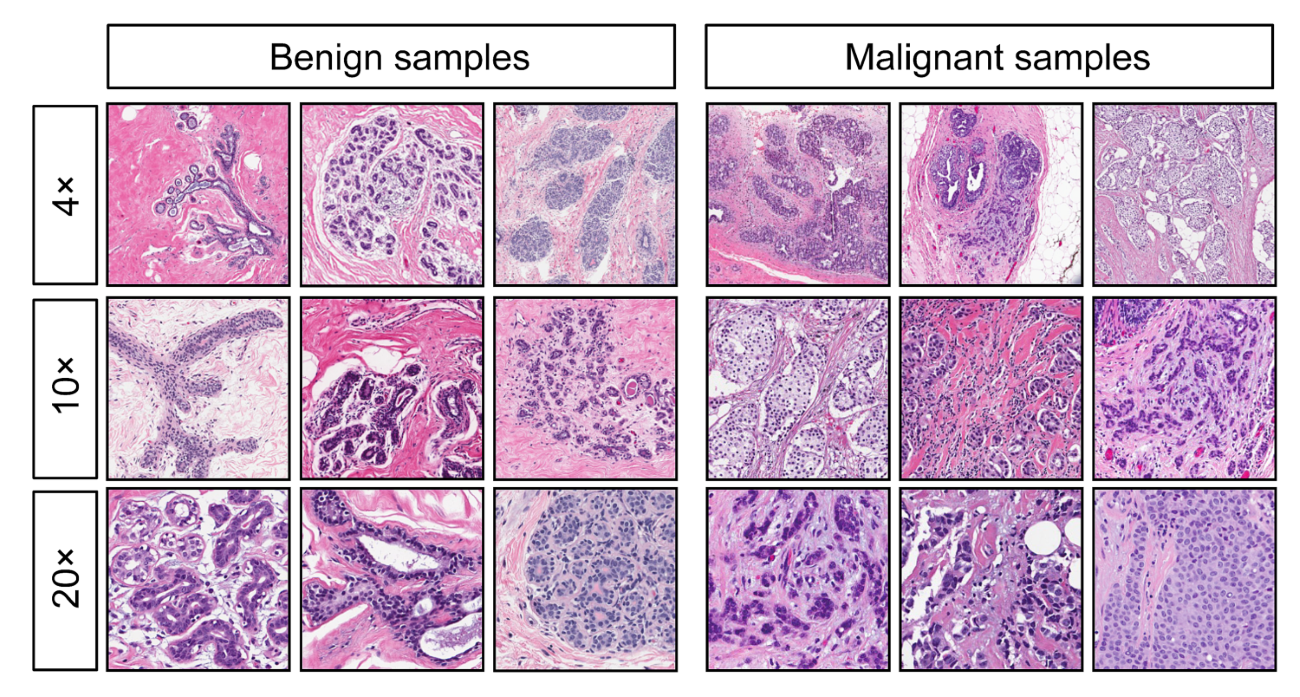
\includegraphics[width=\linewidth]{img/breast_cancer_dataset.png}
            \caption{Breast Cancer Dataset}
         \end{figure}
            \end{column}
        \begin{column}{0.4\textwidth}
            \vspace{1cm}
                \begin{itemize}
        \item 569 samples, 30 features
        \item 50\% train, 50\% test split
        \item Binary classification
    \end{itemize}
        \end{column}


        
    \end{columns}


    
\end{frame}

% Include individual sections
% SVM slides
\input{sections/nonlinear_algo/1_svm_slide}

% Random Forest slides
\input{sections/nonlinear_algo/2_random_forest_slide}

% Gradient Boosting slides
\input{sections/nonlinear_algo/3_gradient_boosting_slide}

% Comparison and Summary
% \input{sections/nonlinear_algo/4_comparison_summary}

% % Final recommendations frame
% \begin{frame}[shrink=10]{Hướng dẫn Lựa chọn Thực tế}
%     \begin{columns}[T]
%         \begin{column}{0.5\textwidth}
%             \begin{exampleblock}{Scenario 1: Không biết bắt đầu}
%                 \begin{itemize}
%                     \item \textbf{Hành động}: Dùng \textbf{Random Forest}
%                     \item Đơn giản, nhanh, không cần chuẩn hóa
%                     \item Baseline tốt để so sánh
%                 \end{itemize}
%             \end{exampleblock}

%             \begin{exampleblock}{Scenario 2: Cần độ chính xác cao}
%                 \begin{itemize}
%                     \item \textbf{Thử}: Gradient Boosting
%                     \item Tuning: $lr \in \{0.01, 0.05, 0.1\}$
%                     \item Thêm: cross-validation để monitor
%                 \end{itemize}
%             \end{exampleblock}

%             \begin{exampleblock}{Scenario 3: Dữ liệu rất lớn}
%                 \begin{itemize}
%                     \item \textbf{Dùng}: Extra Trees hoặc GB
%                     \item Random Forest quá chậm
%                     \item Xem xét sampling strategies
%                 \end{itemize}
%             \end{exampleblock}
%         \end{column}

%         \begin{column}{0.45\textwidth}
%             \begin{alertblock}{Common Mistakes}
%                 \begin{enumerate}
%                     \item \textbf{Quên chuẩn hóa cho SVM}
%                     \begin{itemize}
%                         \item SVM nhạy cảm với scale
%                         \item StandardScaler là BẮT BUỘC
%                     \end{itemize}
                    
%                     \item \textbf{Vừa tune quá ít cho GB}
%                     \begin{itemize}
%                         \item $lr$ quá cao: thiếu học
%                         \item $lr$ quá thấp: chậm hội tụ
%                     \end{itemize}
                    
%                     \item \textbf{Không kiểm tra overfitting}
%                     \begin{itemize}
%                         \item Luôn dùng validation set
%                         \item Cross-validation là lợi ích
%                     \end{itemize}
%                 \end{enumerate}
%             \end{alertblock}

%             \begin{block}{Next Steps}
%                 \begin{itemize}
%                     \item Implement trên dữ liệu của bạn
%                     \item Grid search trên hyperparameters
%                     \item So sánh với baseline (e.g., logistic regression)
%                     \item Diễn giải results (feature importance, etc.)
%                 \end{itemize}
%             \end{block}
%         \end{column}
%     \end{columns}

%     \hfill{\scriptsize \cite{duchesnay2021statsml}}
% \end{frame}


\section{Non-linear Learning Algorithms}

% Introduction frame
\begin{frame}{Non-linear Learning Algorithms: Tổng Quan}
            \begin{enumerate}
                \item \textbf{Support Vector Machines (SVM)}
                \begin{itemize}
                    \item Kernel methods, RBF kernel
                \end{itemize}
                
                \item \textbf{Ensemble Tree Methods}
                \begin{itemize}
                    \item Random Forest, Extra Trees
                \end{itemize}
                
                \item \textbf{Gradient Boosting}
                \begin{itemize}
                    \item Sequential weak learners
                \end{itemize}
            \end{enumerate}

            % \begin{alertblock}{Trade-offs}
            %     \begin{itemize}
            %         \item \textbf{Accuracy}: SVM > GB > RF > ET
            %         \item \textbf{Speed}: ET > RF > GB > SVM
            %         \item \textbf{Interpretability}: Tree > SVM
            %         \item \textbf{Scaling}: ET/RF > GB > SVM
            %     \end{itemize}
            % \end{alertblock}
\end{frame}

\begin{frame}{Benchmark Dataset: Breast Cancer Classification}

    \begin{columns}[T]
        \begin{column}{0.6\textwidth}
         \begin{figure}
            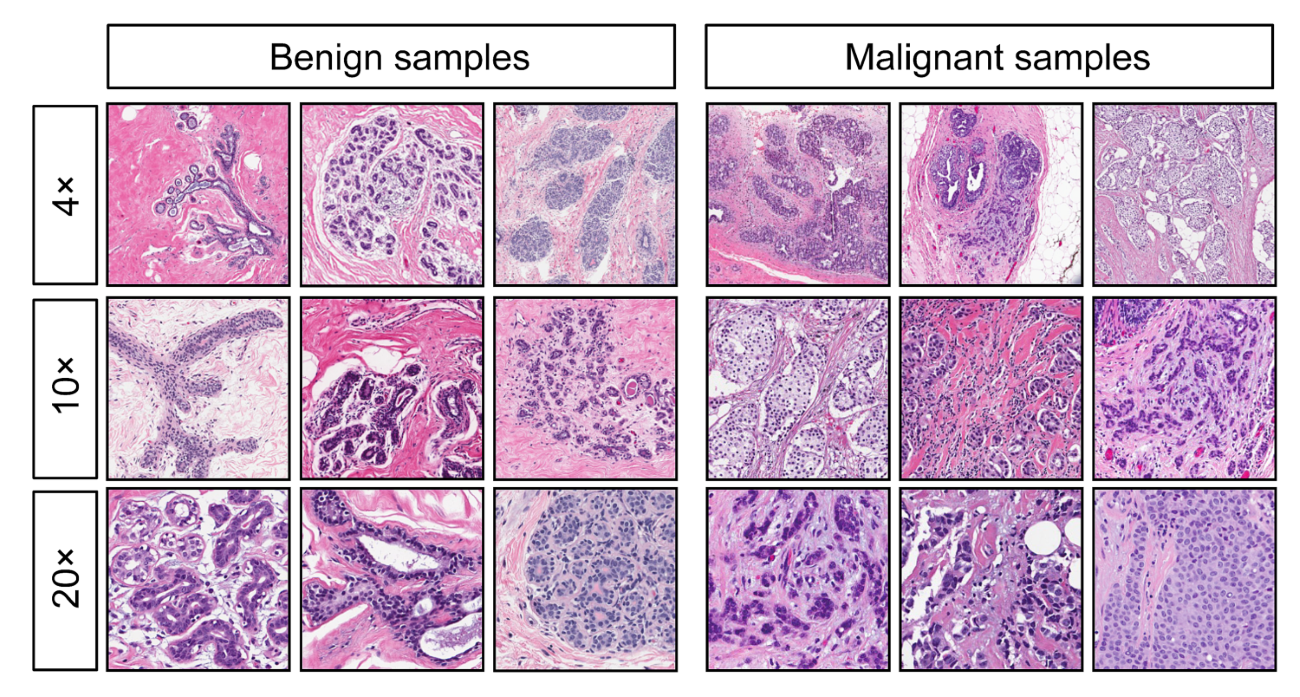
\includegraphics[width=\linewidth]{img/breast_cancer_dataset.png}
            \caption{Breast Cancer Dataset}
         \end{figure}
            \end{column}
        \begin{column}{0.4\textwidth}
            \vspace{1cm}
                \begin{itemize}
        \item 569 samples, 30 features
        \item 50\% train, 50\% test split
        \item Binary classification
    \end{itemize}
        \end{column}


        
    \end{columns}


    
\end{frame}

% Include individual sections
% SVM slides
\begin{frame}{SVM: Khác gì giữa Linear và Kernel?}
    \begin{columns}
        \begin{column}{0.42\textwidth}
        \textbf{Linear SVM}:\\
            - Tìm một đường thẳng (hoặc siêu phẳng) để phân chia dữ liệu\\
            - Hoạt động trực tiếp trên dữ liệu gốc $x$\\
            - Phù hợp khi dữ liệu \textbf{có thể tách tuyến tính}
        \end{column}

        \begin{column}{0.57\textwidth}
        \textbf{Kernel SVM}:\\
            - Dùng \textbf{kernel} để biến dữ liệu sang không gian khác\\
            - Giúp tạo ra \textbf{đường phân chia cong} (phi tuyến)\\
            - Phù hợp khi dữ liệu \textbf{không tách được bằng đường thẳng}
        \end{column}
    \end{columns}

    \begin{alertblock}{Vì sao cần Kernel?}
        Thay vì biến đổi dữ liệu sang không gian nhiều chiều (rất tốn chi phí),
        ta chỉ cần tính \textbf{độ giống nhau} giữa hai điểm bằng hàm $K(x_i, x_j)$.\\
        Kernel Trick giúp:
        \begin{itemize}
            \item Xử lý được dữ liệu phi tuyến
            \item Không cần thực sự tính toán trong không gian cao chiều
            \item Giữ chi phí tính toán thấp hơn
        \end{itemize}
        % Đã xóa thẻ \end{itemize} bị thừa ở đây
    \end{alertblock}

    \vspace{0.2cm}

    \textbf{Hàm quyết định:}
    \[
        f(x) = \operatorname{sign}\left(\sum_i \alpha_i y_i K(x_i, x) + b\right)
    \]
\end{frame}

\begin{frame}{RBF Kernel: điểm khác biệt chính với Linear SVM}
                  Kernel được sử dụng phổ biến nhất là RBF kernel:
                \[
                    K(x_i, x_j) = \exp\left(-\frac{\|x_i - x_j\|^2}{2\sigma^2}\right)
                \]
                hoặc viết lại:
                \[
                    K(x_i, x_j) = \exp\left(-\gamma \|x_i - x_j\|^2\right)
                \]
    \begin{columns}[T]
        \begin{column}{0.48\textwidth}
            \begin{alertblock}{Ý nghĩa hình học}
                \begin{itemize}
                    \item Hàm Gaussian tâm ở mỗi điểm dữ liệu $x_i$
                    \item Độ tương tự giảm theo khoảng cách Euclid bình phương
                    \item $\sigma$ điều khiển độ rộng kernel
                \end{itemize}
            \end{alertblock}
        \end{column}

        \begin{column}{0.48\textwidth}

            \begin{block}{Lợi ích RBF}
                \begin{itemize}
                    \item Linh hoạt cho các bài toán phi tuyến
                    \item Dễ cài đặt và tối chỉnh
                    \item Hoạt động tốt với dữ liệu nhiều chiều
                \end{itemize}
                \vspace{0.5cm}
            \end{block}
        \end{column}
    \end{columns}

    \hfill{\scriptsize \cite{duchesnay2021statsml}}
\end{frame}

\begin{frame}[shrink=10]{SVM: Đánh giá}
            \begin{columns}[T]
                \begin{column}{0.48\textwidth}
                    \textbf{Ưu điểm:}
                    \begin{itemize}
                        \item Hiệu quả với dữ liệu nhiều chiều, biên phân tách rõ
                        \item Tổng quát hóa tốt nhờ tối ưu margin
                        \item Kết hợp kernel để xử lý quan hệ phi tuyến
                    \end{itemize}
                \end{column}
                \begin{column}{0.48\textwidth}
                    \textbf{Nhược điểm:}
                    \begin{itemize}
                        \item Nhạy với tham số $C$, $\gamma$ và lựa chọn kernel
                        \item Chi phí huấn luyện cao khi số mẫu lớn
                        \item Khó diễn giải trực quan hơn một số mô hình tuyến tính
                    \end{itemize}
                \end{column}
            \end{columns}

            \begin{alertblock}{Kết quả mẫu (Breast Cancer)}
                Sử dụng RBF kernel + StandardScaler:
                \begin{itemize}
                    \item \textbf{bAcc}: 0.97 (Balanced Accuracy)
                    \item \textbf{AUC}: 0.99 (công thức)
                    \item \textbf{AUC}: 0.99 (xác suất)
                \end{itemize}
            \end{alertblock}

    \hfill{\scriptsize \cite{duchesnay2021statsml}}
\end{frame}


% Random Forest slides
\begin{frame}{Decision Trees: Nền tảng của Random Forest}
    \begin{columns}[T]
        \begin{column}{0.55\textwidth}
                Decision Tree học bằng cách chia dữ liệu theo các điều kiện trên đặc trưng:
                \begin{itemize}
                    \item Mỗi nút là một phép thử
                    \item Chọn split tốt nhất theo Gini/Entropy
                    \item Lặp lại đến khi nút đủ ``thuần'' hoặc đạt điều kiện dừng
                \end{itemize}

        \end{column}

        \begin{column}{0.4\textwidth}
                \centering
                % \fbox{\parbox[c][2.9cm][c]{0.9\linewidth}{\centering Ch\`en \h`inh minh h\d{o}a Decision Tree v\`ao \^o n\`ay}}
                % Sau khi co anh, co the thay bang:
                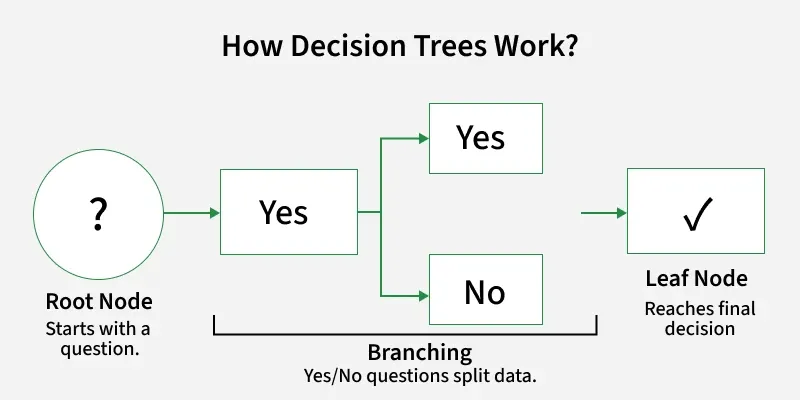
\includegraphics[width=0.95\linewidth]{img/how_decision_trees_work_.png}
        \end{column}
    \end{columns}

                \begin{alertblock}{Vấn đề chính}
                \textbf{Decision Trees dễ overfitting}!
                \begin{itemize}
                    \item Một cây học từ một con đường quyết định duy nhất
                    \item Không dự báo tốt trên dữ liệu mới
                    \item Phương pháp khắc phục: \textbf{Random Forest}
                \end{itemize}
            \end{alertblock}
\end{frame}

\begin{frame}[shrink=8]{Random Forest: Giảm Overfitting}

                Random Forest là một bộ ước lượng tổng quát được phát triển bởi Leo Breiman để giảm overfitting:
                \begin{itemize}
                    \item Xây dựng \textbf{nhiều cây quyết định}
                    \item Trên các \textbf{mẫu con khác nhau} của dữ liệu
                    \item Sử dụng \textbf{trung bình hóa} để cải thiện độ chính xác
                \end{itemize}

            \begin{block}{Giảm Overfitting: Quy trình}
                \begin{itemize}
                    \item Tạo $n\_estimators$ cây quyết định
                    \item Mỗi cây học trên bootstrap sample (lấy mẫu có hoàn lại)
                    \item Mỗi nút chỉ xét tập con ngẫu nhiên của đặc trưng
                    \item Dự đoán cuối: vote (phân loại) hoặc trung bình (hồi quy)
                \end{itemize}
            \end{block}
\end{frame}

\begin{frame}[shrink=10]{Random Forest vs Extra Trees: Sự khác biệt}
    \centering
    \begin{tabular}{p{0.22\linewidth} p{0.35\linewidth} p{0.35\linewidth}}
        \toprule
        \textbf{Tiêu chí} & \textbf{Random Forest} & \textbf{Extra Trees} \\
        \midrule
        \textbf{Bootstrap sampling} & Có (lấy mẫu có hoàn lại) & Không (lấy mẫu có hoàn lại) \\
        \textbf{Cách chọn split} & Chọn best split ở mỗi nút & Chọn split ngẫu nhiên ở mỗi nút \\
        \textbf{Phương sai} & Cao hơn & Thấp hơn \\
        \textbf{Bias} & Thấp hơn & Cao hơn \\
        \textbf{Tốc độ} & Chậm hơn (phải tìm best split) & Nhanh hơn (random split) \\
        \bottomrule
    \end{tabular}
    \vspace{0.2cm}
    
    \begin{alertblock}{Lưu ý}
        \textbf{ExtraTrees} được gọi là ``Extremely Randomized Trees''. Nó dùng random splits thay vì best splits để giảm phương sai, nhưng tăng bias.
    \end{alertblock}
\end{frame}

\begin{frame}[shrink=10]{Random Forest: Đánh giá}
    \begin{columns}[T]
        \begin{column}{0.48\textwidth}
            \textbf{Ưu điểm:}
            \begin{itemize}
                \item Giảm overfitting tốt hơn cây đơn lẻ
                \item Ổn định nhờ trung bình hóa nhiều cây
                \item Ít cần chuẩn hóa dữ liệu đầu vào
            \end{itemize}
        \end{column}
        \begin{column}{0.48\textwidth}
            \textbf{Nhược điểm:}
            \begin{itemize}
                \item Khó diễn giải hơn Decision Tree
                \item Chi phí suy luận tăng khi số cây lớn
                \item Có thể kém hơn SVM ở một số bài toán biên rõ
            \end{itemize}
        \end{column}
    \end{columns}

    \begin{alertblock}{Kết quả mẫu (Breast Cancer)}
        Cấu hình: \texttt{n\_estimators=100}, train/test split $50\%$:
        \begin{itemize}
            \item \textbf{bAcc}: 0.93
            \item \textbf{AUC}: 0.98
            \item So với SVM (bAcc=0.97, AUC=0.99): thấp hơn nhẹ nhưng dễ dùng
        \end{itemize}
    \end{alertblock}

    \hfill{\scriptsize \cite{duchesnay2021statsml}}
\end{frame}


% Gradient Boosting slides
\begin{frame}{Gradient Boosting: Khái niệm Cơ bản}
    \begin{columns}[T]
        \begin{column}{0.59\textwidth}
            Gradient Boosting xây dựng chuỗi bộ học yếu theo kiểu tuần tự:
            \begin{itemize}
                \item Mô hình sau học từ lỗi của mô hình trước
                \item Tối ưu dần phần dư (residuals)
                \item Dự đoán cuối là tổng có trọng số
            \end{itemize}
        \end{column}

        \begin{column}{0.4\textwidth}
            \centering
            % \fbox{\parbox[c][2.9cm][c]{0.9\linewidth}{\centering Ch\`en h\`inh minh h\d{o}a chu\~oi boosting v\`ao \^o n\`ay}}
            % Sau khi co anh, co the thay bang:
            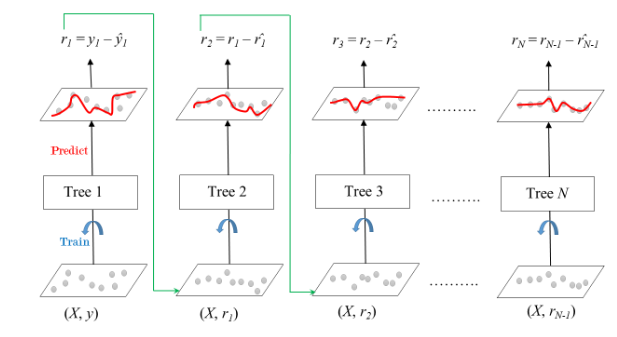
\includegraphics[width=0.95\linewidth]{img/gradientboosting.png}
        \end{column}
    \end{columns}

                \begin{block}{Ý tưởng chính}
                \begin{enumerate}
                    \item Huấn luyện mô hình đầu tiên
                    \item Tính sai số còn lại
                    \item Huấn luyện mô hình mới để sửa sai số đó
                \end{enumerate}
            \end{block}
\end{frame}

\begin{frame}{Gradient Boosting: Quy trình và Tuning}
                \begin{itemize}
                    \item Khởi tạo mô hình yếu ban đầu
                    \item Với mỗi vòng lặp: học trên residuals
                    \item Cập nhật: $f_t(x) = f_{t-1}(x) + lr \cdot h_t(x)$
                    \item Lặp đến $n\_estimators$
                \end{itemize}

            \begin{block}{Regularization chính}
                \begin{itemize}
                    \item \textbf{learning\_rate}: nhỏ hơn $\Rightarrow$ học chậm, ổn định hơn
                    \item \textbf{subsample} $< 1$: Stochastic GB, giảm overfitting
                \end{itemize}
            \end{block}
\end{frame}

\begin{frame}[shrink=10]{Gradient Boosting: Đánh giá}
    \begin{columns}[T]
        \begin{column}{0.48\textwidth}
            \textbf{Ưu điểm:}
            \begin{itemize}
                \item Độ chính xác cao trên dữ liệu có pattern phức tạp
                \item Tập trung sửa lỗi từng bước
                \item Linh hoạt với nhiều hàm mất mát
            \end{itemize}
        \end{column}
        \begin{column}{0.48\textwidth}
            \textbf{Nhược điểm:}
            \begin{itemize}
                \item Dễ overfitting nếu tuning chưa tốt
                \item Huấn luyện chậm hơn Bagging do tính tuần tự
                \item Nhạy với hyperparameters
            \end{itemize}
        \end{column}
    \end{columns}

    \begin{alertblock}{Kết quả mẫu (Breast Cancer)}
        Cấu hình: $n\_estimators=100$, $learning\_rate=0.1$, $subsample=0.5$:
        \begin{itemize}
            \item \textbf{bAcc}: 0.94
            \item \textbf{AUC}: 0.98
            \item So với SVM: thấp hơn nhẹ; so với RF: nhỉnh hơn bAcc
        \end{itemize}
    \end{alertblock}

    \hfill{\scriptsize \cite{duchesnay2021statsml}}
\end{frame}


% Comparison and Summary
% \begin{frame}{Tổng quan: So sánh các Phương pháp Non-linear}
    \footnotesize
    \renewcommand{\arraystretch}{1.3}
    \begin{tabular}{p{0.16\linewidth} p{0.2\linewidth} p{0.2\linewidth} p{0.2\linewidth} p{0.15\linewidth}}
        \toprule
        \textbf{Khía cạnh} & \textbf{SVM (RBF)} & \textbf{Random Forest} & \textbf{Gradient Boosting} & \textbf{Extra Trees} \\
        \midrule
        \textbf{Kernel/} & Kernel trick & Tree ensemble & Seq. weak & Tree ensemble \\
        \textbf{Cơ chế} & (kernel space) & (Bagging) & learners & (random split) \\
        &  &  &  &  \\
        
        \textbf{Chuẩn hóa} & \textbf{BẮT BUỘC} & Không cần & Không cần & Không cần \\
        \textbf{dữ liệu} & (StandardScaler) & &  &  \\
        &  &  &  &  \\
        
        \textbf{Độ chính xác} & \textbf{0.97} (bAcc) & \textbf{0.93} & \textbf{0.94} & \textbf{~ 0.92} \\
        (Breast Cancer) & \textbf{0.99} (AUC) & \textbf{0.98} & \textbf{0.98} & (estimated) \\
        &  &  &  &  \\
        
        \textbf{Tốc độ học} & Chậm-Trung & Nhanh & Chậm & \textbf{Rất nhanh} \\
        \textbf{Tốc độ dự đoán} & Trung & Nhanh & Chậm & Nhanh \\
        &  &  &  &  \\
        
        \textbf{Diễn giải} & Khó & Dễ & Trung & Dễ \\
        &  &  &  &  \\
        
        \textbf{Overfitting} & Tuning $\gamma$ & Tuning depth & Tuning $lr$, & Tuning split \\
        \textbf{Kiểm soát} & C & n\_estimators & subsample & n\_estimators \\
        &  &  &  &  \\
        
        \textbf{Khi nào} & Msr-sized, & Large, & Very large, & Cần tốc độ \\
        \textbf{dùng} & cần SVM & interpretability & best accuracy & or CPU \\
        &  &  &  &  \\
        \bottomrule
    \end{tabular}

    \vspace{0.2cm}
    \begin{alertblock}{Khuyến cáo}
        \begin{itemize}
            \item \textbf{Start với Random Forest}: dễ, nhanh, không cần tuning phức tạp
            \item \textbf{Gradient Boosting} nếu cần tăng từ 0.93 đến 0.94-0.95: tốt hơn nhưng tuning khó hơn
            \item \textbf{SVM}: khi có thời gian tuning, dữ liệu vừa phải đến lớn
            \item \textbf{Extra Trees}: khi cần rất nhanh hoặc dữ liệu massive tới mức RF quá chậm
        \end{itemize}
    \end{alertblock}

    \hfill{\scriptsize \cite{duchesnay2021statsml}}
\end{frame}

% \begin{frame}[shrink=10]{Lựa chọn Phương pháp: Quy tắc Thực hành}
%     \begin{columns}[T]
%         \begin{column}{0.52\textwidth}
%             \begin{block}{Bước 1: Kích thước Dữ liệu}
%                 \begin{itemize}
%                     \item \textbf{Nhỏ}: $n < 1000$ $\Rightarrow$ SVM hoặc RF
%                     \item \textbf{Vừa}: $1000 < n < 100k$ $\Rightarrow$ Tất cả phù hợp
%                     \item \textbf{Lớn}: $n > 100k$ $\Rightarrow$ RF, GB, Extra Trees
%                 \end{itemize}
%             \end{block}

%             \begin{block}{Bước 2: Yêu cầu về Tốc độ}
%                 \begin{itemize}
%                     \item \textbf{Học online/Real-time}: Extra Trees
%                     \item \textbf{Batch, không yêu cầu}: GB (tuning riêm mỹ)
%                     \item \textbf{Cân bằng}: Random Forest
%                 \end{itemize}
%             \end{block}

%             \begin{block}{Bước 3: Interpretability}
%                 \begin{itemize}
%                     \item \textbf{Cần diễn giải}: RF, Extra Trees, Shallow GB
%                     \item \textbf{Không yêu cầu}: SVM, Deep GB
%                 \end{itemize}
%             \end{block}
%         \end{column}

%         \begin{column}{0.44\textwidth}
%             \begin{exampleblock}{Luồng quyết định}
%                 \begin{enumerate}
%                     \item Dữ liệu lớn $(n > 100k)$?
%                     \begin{itemize}
%                         \item YES $\Rightarrow$ Extra Trees (tốc độ)
%                         \item NO $\Rightarrow$ Bước 2
%                     \end{itemize}
                    
%                     \item Cần diễn giải?
%                     \begin{itemize}
%                         \item YES $\Rightarrow$ Random Forest
%                         \item NO $\Rightarrow$ Bước 3
%                     \end{itemize}
                    
%                     \item Compact/Tuning Expertise?
%                     \begin{itemize}
%                         \item YES $\Rightarrow$ SVM + GB
%                         \item NO $\Rightarrow$ Random Forest
%                     \end{itemize}
%                 \end{enumerate}
%             \end{exampleblock}

%             \begin{alertblock}{Golden Rule}
%                 \textbf{Bắt đầu với Random Forest}, sau đó thử GB/SVM nếu cần chút tăng độ chính xác.
%             \end{alertblock}
%         \end{column}
%     \end{columns}

%     \hfill{\scriptsize \cite{duchesnay2021statsml}}
% \end{frame}

% \begin{frame}[shrink=12]{Các Điểm Chính - Tóm Lược}
%     \begin{columns}[T]
%         \begin{column}{0.48\textwidth}
%             \begin{block}{Support Vector Machines}
%                 \begin{itemize}
%                     \item Kernel trick: tính toán hiệu quả trong cao chiều
%                     \item RBF kernel phổ biến nhất (Gaussian)
%                     \item \textbf{Bắt buộc chuẩn hóa} dữ liệu
%                     \item Decision function: $\sum \alpha_i y_i K(x_i, x)$
%                     \item Kết quả: bAcc=0.97, AUC=0.99
%                 \end{itemize}
%             \end{block}

%             \begin{block}{Random Forest \& Extra Trees}
%                 \begin{itemize}
%                     \item Ensemble của decision trees
%                     \item RF: bootstrap + best split
%                     \item ET: no bootstrap + random split
%                     \item RF tốt hơn nhưng chậm hơn ET
%                     \item Không cần chuẩn hóa
%                     \item kết quả: bAcc=0.93, AUC=0.98
%                 \end{itemize}
%             \end{block}
%         \end{column}

%         \begin{column}{0.48\textwidth}
%             \begin{block}{Gradient Boosting}
%                 \begin{itemize}
%                     \item Sequential: mỗi cây giảm lỗi của cây trước
%                     \item Hai hyperparameter chính:
%                     \begin{itemize}
%                         \item Learning rate: kiểm soát tốc độ
%                         \item Subsample: stochastic gradient boosting
%                     \end{itemize}
%                     \item Regularization hiệu quả
%                     \item Không cần chuẩn hóa
%                     \item Kết quả: bAcc=0.94, AUC=0.98
%                 \end{itemize}
%             \end{block}

%             \begin{exampleblock}{Khuyến cáo Chung}
%                 \begin{enumerate}
%                     \item Bắt đầu \textbf{Random Forest}
%                     \item Thử \textbf{Gradient Boosting} để tăng chút xíu
%                     \item \textbf{SVM} nếu có thời gian tuning
%                     \item \textbf{Extra Trees} cho tốc độ cực đại
%                 \end{enumerate}
%             \end{exampleblock}
%         \end{column}
%     \end{columns}

%     \hfill{\scriptsize \cite{duchesnay2021statsml}}
% \end{frame}


% % Final recommendations frame
% \begin{frame}[shrink=10]{Hướng dẫn Lựa chọn Thực tế}
%     \begin{columns}[T]
%         \begin{column}{0.5\textwidth}
%             \begin{exampleblock}{Scenario 1: Không biết bắt đầu}
%                 \begin{itemize}
%                     \item \textbf{Hành động}: Dùng \textbf{Random Forest}
%                     \item Đơn giản, nhanh, không cần chuẩn hóa
%                     \item Baseline tốt để so sánh
%                 \end{itemize}
%             \end{exampleblock}

%             \begin{exampleblock}{Scenario 2: Cần độ chính xác cao}
%                 \begin{itemize}
%                     \item \textbf{Thử}: Gradient Boosting
%                     \item Tuning: $lr \in \{0.01, 0.05, 0.1\}$
%                     \item Thêm: cross-validation để monitor
%                 \end{itemize}
%             \end{exampleblock}

%             \begin{exampleblock}{Scenario 3: Dữ liệu rất lớn}
%                 \begin{itemize}
%                     \item \textbf{Dùng}: Extra Trees hoặc GB
%                     \item Random Forest quá chậm
%                     \item Xem xét sampling strategies
%                 \end{itemize}
%             \end{exampleblock}
%         \end{column}

%         \begin{column}{0.45\textwidth}
%             \begin{alertblock}{Common Mistakes}
%                 \begin{enumerate}
%                     \item \textbf{Quên chuẩn hóa cho SVM}
%                     \begin{itemize}
%                         \item SVM nhạy cảm với scale
%                         \item StandardScaler là BẮT BUỘC
%                     \end{itemize}
                    
%                     \item \textbf{Vừa tune quá ít cho GB}
%                     \begin{itemize}
%                         \item $lr$ quá cao: thiếu học
%                         \item $lr$ quá thấp: chậm hội tụ
%                     \end{itemize}
                    
%                     \item \textbf{Không kiểm tra overfitting}
%                     \begin{itemize}
%                         \item Luôn dùng validation set
%                         \item Cross-validation là lợi ích
%                     \end{itemize}
%                 \end{enumerate}
%             \end{alertblock}

%             \begin{block}{Next Steps}
%                 \begin{itemize}
%                     \item Implement trên dữ liệu của bạn
%                     \item Grid search trên hyperparameters
%                     \item So sánh với baseline (e.g., logistic regression)
%                     \item Diễn giải results (feature importance, etc.)
%                 \end{itemize}
%             \end{block}
%         \end{column}
%     \end{columns}

%     \hfill{\scriptsize \cite{duchesnay2021statsml}}
% \end{frame}


\section{Non-linear Learning Algorithms}

% Introduction frame
\begin{frame}{Non-linear Learning Algorithms: Tổng Quan}
            \begin{enumerate}
                \item \textbf{Support Vector Machines (SVM)}
                \begin{itemize}
                    \item Kernel methods, RBF kernel
                \end{itemize}
                
                \item \textbf{Ensemble Tree Methods}
                \begin{itemize}
                    \item Random Forest, Extra Trees
                \end{itemize}
                
                \item \textbf{Gradient Boosting}
                \begin{itemize}
                    \item Sequential weak learners
                \end{itemize}
            \end{enumerate}

            % \begin{alertblock}{Trade-offs}
            %     \begin{itemize}
            %         \item \textbf{Accuracy}: SVM > GB > RF > ET
            %         \item \textbf{Speed}: ET > RF > GB > SVM
            %         \item \textbf{Interpretability}: Tree > SVM
            %         \item \textbf{Scaling}: ET/RF > GB > SVM
            %     \end{itemize}
            % \end{alertblock}
\end{frame}

\begin{frame}{Benchmark Dataset: Breast Cancer Classification}

    \begin{columns}[T]
        \begin{column}{0.6\textwidth}
         \begin{figure}
            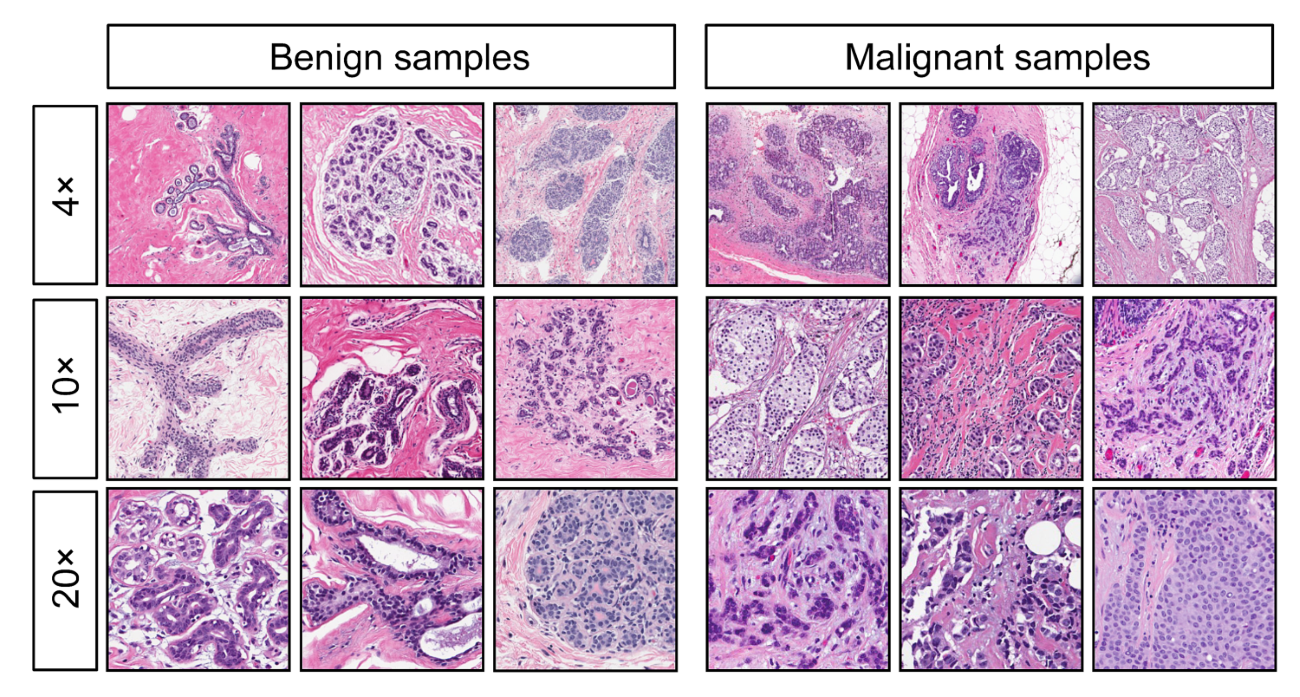
\includegraphics[width=\linewidth]{img/breast_cancer_dataset.png}
            \caption{Breast Cancer Dataset}
         \end{figure}
            \end{column}
        \begin{column}{0.4\textwidth}
            \vspace{1cm}
                \begin{itemize}
        \item 569 samples, 30 features
        \item 50\% train, 50\% test split
        \item Binary classification
    \end{itemize}
        \end{column}


        
    \end{columns}


    
\end{frame}

% Include individual sections
% SVM slides
\begin{frame}{SVM: Khác gì giữa Linear và Kernel?}
    \begin{columns}
        \begin{column}{0.42\textwidth}
        \textbf{Linear SVM}:\\
            - Tìm một đường thẳng (hoặc siêu phẳng) để phân chia dữ liệu\\
            - Hoạt động trực tiếp trên dữ liệu gốc $x$\\
            - Phù hợp khi dữ liệu \textbf{có thể tách tuyến tính}
        \end{column}

        \begin{column}{0.57\textwidth}
        \textbf{Kernel SVM}:\\
            - Dùng \textbf{kernel} để biến dữ liệu sang không gian khác\\
            - Giúp tạo ra \textbf{đường phân chia cong} (phi tuyến)\\
            - Phù hợp khi dữ liệu \textbf{không tách được bằng đường thẳng}
        \end{column}
    \end{columns}

    \begin{alertblock}{Vì sao cần Kernel?}
        Thay vì biến đổi dữ liệu sang không gian nhiều chiều (rất tốn chi phí),
        ta chỉ cần tính \textbf{độ giống nhau} giữa hai điểm bằng hàm $K(x_i, x_j)$.\\
        Kernel Trick giúp:
        \begin{itemize}
            \item Xử lý được dữ liệu phi tuyến
            \item Không cần thực sự tính toán trong không gian cao chiều
            \item Giữ chi phí tính toán thấp hơn
        \end{itemize}
        % Đã xóa thẻ \end{itemize} bị thừa ở đây
    \end{alertblock}

    \vspace{0.2cm}

    \textbf{Hàm quyết định:}
    \[
        f(x) = \operatorname{sign}\left(\sum_i \alpha_i y_i K(x_i, x) + b\right)
    \]
\end{frame}

\begin{frame}{RBF Kernel: điểm khác biệt chính với Linear SVM}
                  Kernel được sử dụng phổ biến nhất là RBF kernel:
                \[
                    K(x_i, x_j) = \exp\left(-\frac{\|x_i - x_j\|^2}{2\sigma^2}\right)
                \]
                hoặc viết lại:
                \[
                    K(x_i, x_j) = \exp\left(-\gamma \|x_i - x_j\|^2\right)
                \]
    \begin{columns}[T]
        \begin{column}{0.48\textwidth}
            \begin{alertblock}{Ý nghĩa hình học}
                \begin{itemize}
                    \item Hàm Gaussian tâm ở mỗi điểm dữ liệu $x_i$
                    \item Độ tương tự giảm theo khoảng cách Euclid bình phương
                    \item $\sigma$ điều khiển độ rộng kernel
                \end{itemize}
            \end{alertblock}
        \end{column}

        \begin{column}{0.48\textwidth}

            \begin{block}{Lợi ích RBF}
                \begin{itemize}
                    \item Linh hoạt cho các bài toán phi tuyến
                    \item Dễ cài đặt và tối chỉnh
                    \item Hoạt động tốt với dữ liệu nhiều chiều
                \end{itemize}
                \vspace{0.5cm}
            \end{block}
        \end{column}
    \end{columns}

    \hfill{\scriptsize \cite{duchesnay2021statsml}}
\end{frame}

\begin{frame}[shrink=10]{SVM: Đánh giá}
            \begin{columns}[T]
                \begin{column}{0.48\textwidth}
                    \textbf{Ưu điểm:}
                    \begin{itemize}
                        \item Hiệu quả với dữ liệu nhiều chiều, biên phân tách rõ
                        \item Tổng quát hóa tốt nhờ tối ưu margin
                        \item Kết hợp kernel để xử lý quan hệ phi tuyến
                    \end{itemize}
                \end{column}
                \begin{column}{0.48\textwidth}
                    \textbf{Nhược điểm:}
                    \begin{itemize}
                        \item Nhạy với tham số $C$, $\gamma$ và lựa chọn kernel
                        \item Chi phí huấn luyện cao khi số mẫu lớn
                        \item Khó diễn giải trực quan hơn một số mô hình tuyến tính
                    \end{itemize}
                \end{column}
            \end{columns}

            \begin{alertblock}{Kết quả mẫu (Breast Cancer)}
                Sử dụng RBF kernel + StandardScaler:
                \begin{itemize}
                    \item \textbf{bAcc}: 0.97 (Balanced Accuracy)
                    \item \textbf{AUC}: 0.99 (công thức)
                    \item \textbf{AUC}: 0.99 (xác suất)
                \end{itemize}
            \end{alertblock}

    \hfill{\scriptsize \cite{duchesnay2021statsml}}
\end{frame}


% Random Forest slides
\begin{frame}{Decision Trees: Nền tảng của Random Forest}
    \begin{columns}[T]
        \begin{column}{0.55\textwidth}
                Decision Tree học bằng cách chia dữ liệu theo các điều kiện trên đặc trưng:
                \begin{itemize}
                    \item Mỗi nút là một phép thử
                    \item Chọn split tốt nhất theo Gini/Entropy
                    \item Lặp lại đến khi nút đủ ``thuần'' hoặc đạt điều kiện dừng
                \end{itemize}

        \end{column}

        \begin{column}{0.4\textwidth}
                \centering
                % \fbox{\parbox[c][2.9cm][c]{0.9\linewidth}{\centering Ch\`en \h`inh minh h\d{o}a Decision Tree v\`ao \^o n\`ay}}
                % Sau khi co anh, co the thay bang:
                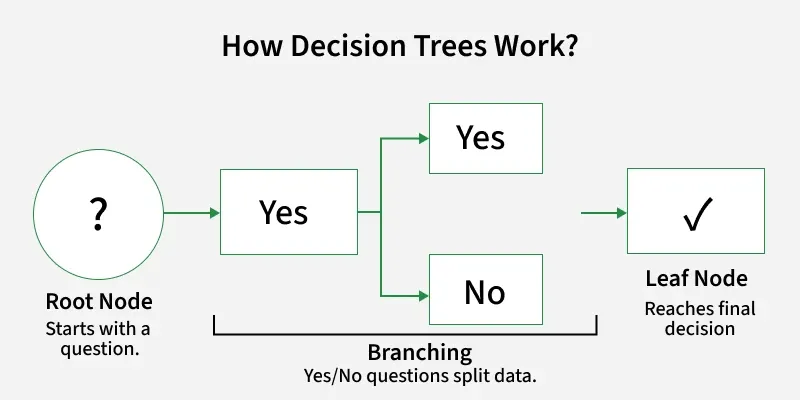
\includegraphics[width=0.95\linewidth]{img/how_decision_trees_work_.png}
        \end{column}
    \end{columns}

                \begin{alertblock}{Vấn đề chính}
                \textbf{Decision Trees dễ overfitting}!
                \begin{itemize}
                    \item Một cây học từ một con đường quyết định duy nhất
                    \item Không dự báo tốt trên dữ liệu mới
                    \item Phương pháp khắc phục: \textbf{Random Forest}
                \end{itemize}
            \end{alertblock}
\end{frame}

\begin{frame}[shrink=8]{Random Forest: Giảm Overfitting}

                Random Forest là một bộ ước lượng tổng quát được phát triển bởi Leo Breiman để giảm overfitting:
                \begin{itemize}
                    \item Xây dựng \textbf{nhiều cây quyết định}
                    \item Trên các \textbf{mẫu con khác nhau} của dữ liệu
                    \item Sử dụng \textbf{trung bình hóa} để cải thiện độ chính xác
                \end{itemize}

            \begin{block}{Giảm Overfitting: Quy trình}
                \begin{itemize}
                    \item Tạo $n\_estimators$ cây quyết định
                    \item Mỗi cây học trên bootstrap sample (lấy mẫu có hoàn lại)
                    \item Mỗi nút chỉ xét tập con ngẫu nhiên của đặc trưng
                    \item Dự đoán cuối: vote (phân loại) hoặc trung bình (hồi quy)
                \end{itemize}
            \end{block}
\end{frame}

\begin{frame}[shrink=10]{Random Forest vs Extra Trees: Sự khác biệt}
    \centering
    \begin{tabular}{p{0.22\linewidth} p{0.35\linewidth} p{0.35\linewidth}}
        \toprule
        \textbf{Tiêu chí} & \textbf{Random Forest} & \textbf{Extra Trees} \\
        \midrule
        \textbf{Bootstrap sampling} & Có (lấy mẫu có hoàn lại) & Không (lấy mẫu có hoàn lại) \\
        \textbf{Cách chọn split} & Chọn best split ở mỗi nút & Chọn split ngẫu nhiên ở mỗi nút \\
        \textbf{Phương sai} & Cao hơn & Thấp hơn \\
        \textbf{Bias} & Thấp hơn & Cao hơn \\
        \textbf{Tốc độ} & Chậm hơn (phải tìm best split) & Nhanh hơn (random split) \\
        \bottomrule
    \end{tabular}
    \vspace{0.2cm}
    
    \begin{alertblock}{Lưu ý}
        \textbf{ExtraTrees} được gọi là ``Extremely Randomized Trees''. Nó dùng random splits thay vì best splits để giảm phương sai, nhưng tăng bias.
    \end{alertblock}
\end{frame}

\begin{frame}[shrink=10]{Random Forest: Đánh giá}
    \begin{columns}[T]
        \begin{column}{0.48\textwidth}
            \textbf{Ưu điểm:}
            \begin{itemize}
                \item Giảm overfitting tốt hơn cây đơn lẻ
                \item Ổn định nhờ trung bình hóa nhiều cây
                \item Ít cần chuẩn hóa dữ liệu đầu vào
            \end{itemize}
        \end{column}
        \begin{column}{0.48\textwidth}
            \textbf{Nhược điểm:}
            \begin{itemize}
                \item Khó diễn giải hơn Decision Tree
                \item Chi phí suy luận tăng khi số cây lớn
                \item Có thể kém hơn SVM ở một số bài toán biên rõ
            \end{itemize}
        \end{column}
    \end{columns}

    \begin{alertblock}{Kết quả mẫu (Breast Cancer)}
        Cấu hình: \texttt{n\_estimators=100}, train/test split $50\%$:
        \begin{itemize}
            \item \textbf{bAcc}: 0.93
            \item \textbf{AUC}: 0.98
            \item So với SVM (bAcc=0.97, AUC=0.99): thấp hơn nhẹ nhưng dễ dùng
        \end{itemize}
    \end{alertblock}

    \hfill{\scriptsize \cite{duchesnay2021statsml}}
\end{frame}


% Gradient Boosting slides
\begin{frame}{Gradient Boosting: Khái niệm Cơ bản}
    \begin{columns}[T]
        \begin{column}{0.59\textwidth}
            Gradient Boosting xây dựng chuỗi bộ học yếu theo kiểu tuần tự:
            \begin{itemize}
                \item Mô hình sau học từ lỗi của mô hình trước
                \item Tối ưu dần phần dư (residuals)
                \item Dự đoán cuối là tổng có trọng số
            \end{itemize}
        \end{column}

        \begin{column}{0.4\textwidth}
            \centering
            % \fbox{\parbox[c][2.9cm][c]{0.9\linewidth}{\centering Ch\`en h\`inh minh h\d{o}a chu\~oi boosting v\`ao \^o n\`ay}}
            % Sau khi co anh, co the thay bang:
            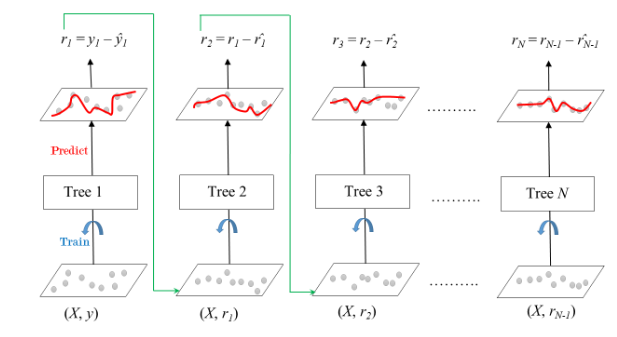
\includegraphics[width=0.95\linewidth]{img/gradientboosting.png}
        \end{column}
    \end{columns}

                \begin{block}{Ý tưởng chính}
                \begin{enumerate}
                    \item Huấn luyện mô hình đầu tiên
                    \item Tính sai số còn lại
                    \item Huấn luyện mô hình mới để sửa sai số đó
                \end{enumerate}
            \end{block}
\end{frame}

\begin{frame}{Gradient Boosting: Quy trình và Tuning}
                \begin{itemize}
                    \item Khởi tạo mô hình yếu ban đầu
                    \item Với mỗi vòng lặp: học trên residuals
                    \item Cập nhật: $f_t(x) = f_{t-1}(x) + lr \cdot h_t(x)$
                    \item Lặp đến $n\_estimators$
                \end{itemize}

            \begin{block}{Regularization chính}
                \begin{itemize}
                    \item \textbf{learning\_rate}: nhỏ hơn $\Rightarrow$ học chậm, ổn định hơn
                    \item \textbf{subsample} $< 1$: Stochastic GB, giảm overfitting
                \end{itemize}
            \end{block}
\end{frame}

\begin{frame}[shrink=10]{Gradient Boosting: Đánh giá}
    \begin{columns}[T]
        \begin{column}{0.48\textwidth}
            \textbf{Ưu điểm:}
            \begin{itemize}
                \item Độ chính xác cao trên dữ liệu có pattern phức tạp
                \item Tập trung sửa lỗi từng bước
                \item Linh hoạt với nhiều hàm mất mát
            \end{itemize}
        \end{column}
        \begin{column}{0.48\textwidth}
            \textbf{Nhược điểm:}
            \begin{itemize}
                \item Dễ overfitting nếu tuning chưa tốt
                \item Huấn luyện chậm hơn Bagging do tính tuần tự
                \item Nhạy với hyperparameters
            \end{itemize}
        \end{column}
    \end{columns}

    \begin{alertblock}{Kết quả mẫu (Breast Cancer)}
        Cấu hình: $n\_estimators=100$, $learning\_rate=0.1$, $subsample=0.5$:
        \begin{itemize}
            \item \textbf{bAcc}: 0.94
            \item \textbf{AUC}: 0.98
            \item So với SVM: thấp hơn nhẹ; so với RF: nhỉnh hơn bAcc
        \end{itemize}
    \end{alertblock}

    \hfill{\scriptsize \cite{duchesnay2021statsml}}
\end{frame}


% Comparison and Summary
% \begin{frame}{Tổng quan: So sánh các Phương pháp Non-linear}
    \footnotesize
    \renewcommand{\arraystretch}{1.3}
    \begin{tabular}{p{0.16\linewidth} p{0.2\linewidth} p{0.2\linewidth} p{0.2\linewidth} p{0.15\linewidth}}
        \toprule
        \textbf{Khía cạnh} & \textbf{SVM (RBF)} & \textbf{Random Forest} & \textbf{Gradient Boosting} & \textbf{Extra Trees} \\
        \midrule
        \textbf{Kernel/} & Kernel trick & Tree ensemble & Seq. weak & Tree ensemble \\
        \textbf{Cơ chế} & (kernel space) & (Bagging) & learners & (random split) \\
        &  &  &  &  \\
        
        \textbf{Chuẩn hóa} & \textbf{BẮT BUỘC} & Không cần & Không cần & Không cần \\
        \textbf{dữ liệu} & (StandardScaler) & &  &  \\
        &  &  &  &  \\
        
        \textbf{Độ chính xác} & \textbf{0.97} (bAcc) & \textbf{0.93} & \textbf{0.94} & \textbf{~ 0.92} \\
        (Breast Cancer) & \textbf{0.99} (AUC) & \textbf{0.98} & \textbf{0.98} & (estimated) \\
        &  &  &  &  \\
        
        \textbf{Tốc độ học} & Chậm-Trung & Nhanh & Chậm & \textbf{Rất nhanh} \\
        \textbf{Tốc độ dự đoán} & Trung & Nhanh & Chậm & Nhanh \\
        &  &  &  &  \\
        
        \textbf{Diễn giải} & Khó & Dễ & Trung & Dễ \\
        &  &  &  &  \\
        
        \textbf{Overfitting} & Tuning $\gamma$ & Tuning depth & Tuning $lr$, & Tuning split \\
        \textbf{Kiểm soát} & C & n\_estimators & subsample & n\_estimators \\
        &  &  &  &  \\
        
        \textbf{Khi nào} & Msr-sized, & Large, & Very large, & Cần tốc độ \\
        \textbf{dùng} & cần SVM & interpretability & best accuracy & or CPU \\
        &  &  &  &  \\
        \bottomrule
    \end{tabular}

    \vspace{0.2cm}
    \begin{alertblock}{Khuyến cáo}
        \begin{itemize}
            \item \textbf{Start với Random Forest}: dễ, nhanh, không cần tuning phức tạp
            \item \textbf{Gradient Boosting} nếu cần tăng từ 0.93 đến 0.94-0.95: tốt hơn nhưng tuning khó hơn
            \item \textbf{SVM}: khi có thời gian tuning, dữ liệu vừa phải đến lớn
            \item \textbf{Extra Trees}: khi cần rất nhanh hoặc dữ liệu massive tới mức RF quá chậm
        \end{itemize}
    \end{alertblock}

    \hfill{\scriptsize \cite{duchesnay2021statsml}}
\end{frame}

% \begin{frame}[shrink=10]{Lựa chọn Phương pháp: Quy tắc Thực hành}
%     \begin{columns}[T]
%         \begin{column}{0.52\textwidth}
%             \begin{block}{Bước 1: Kích thước Dữ liệu}
%                 \begin{itemize}
%                     \item \textbf{Nhỏ}: $n < 1000$ $\Rightarrow$ SVM hoặc RF
%                     \item \textbf{Vừa}: $1000 < n < 100k$ $\Rightarrow$ Tất cả phù hợp
%                     \item \textbf{Lớn}: $n > 100k$ $\Rightarrow$ RF, GB, Extra Trees
%                 \end{itemize}
%             \end{block}

%             \begin{block}{Bước 2: Yêu cầu về Tốc độ}
%                 \begin{itemize}
%                     \item \textbf{Học online/Real-time}: Extra Trees
%                     \item \textbf{Batch, không yêu cầu}: GB (tuning riêm mỹ)
%                     \item \textbf{Cân bằng}: Random Forest
%                 \end{itemize}
%             \end{block}

%             \begin{block}{Bước 3: Interpretability}
%                 \begin{itemize}
%                     \item \textbf{Cần diễn giải}: RF, Extra Trees, Shallow GB
%                     \item \textbf{Không yêu cầu}: SVM, Deep GB
%                 \end{itemize}
%             \end{block}
%         \end{column}

%         \begin{column}{0.44\textwidth}
%             \begin{exampleblock}{Luồng quyết định}
%                 \begin{enumerate}
%                     \item Dữ liệu lớn $(n > 100k)$?
%                     \begin{itemize}
%                         \item YES $\Rightarrow$ Extra Trees (tốc độ)
%                         \item NO $\Rightarrow$ Bước 2
%                     \end{itemize}
                    
%                     \item Cần diễn giải?
%                     \begin{itemize}
%                         \item YES $\Rightarrow$ Random Forest
%                         \item NO $\Rightarrow$ Bước 3
%                     \end{itemize}
                    
%                     \item Compact/Tuning Expertise?
%                     \begin{itemize}
%                         \item YES $\Rightarrow$ SVM + GB
%                         \item NO $\Rightarrow$ Random Forest
%                     \end{itemize}
%                 \end{enumerate}
%             \end{exampleblock}

%             \begin{alertblock}{Golden Rule}
%                 \textbf{Bắt đầu với Random Forest}, sau đó thử GB/SVM nếu cần chút tăng độ chính xác.
%             \end{alertblock}
%         \end{column}
%     \end{columns}

%     \hfill{\scriptsize \cite{duchesnay2021statsml}}
% \end{frame}

% \begin{frame}[shrink=12]{Các Điểm Chính - Tóm Lược}
%     \begin{columns}[T]
%         \begin{column}{0.48\textwidth}
%             \begin{block}{Support Vector Machines}
%                 \begin{itemize}
%                     \item Kernel trick: tính toán hiệu quả trong cao chiều
%                     \item RBF kernel phổ biến nhất (Gaussian)
%                     \item \textbf{Bắt buộc chuẩn hóa} dữ liệu
%                     \item Decision function: $\sum \alpha_i y_i K(x_i, x)$
%                     \item Kết quả: bAcc=0.97, AUC=0.99
%                 \end{itemize}
%             \end{block}

%             \begin{block}{Random Forest \& Extra Trees}
%                 \begin{itemize}
%                     \item Ensemble của decision trees
%                     \item RF: bootstrap + best split
%                     \item ET: no bootstrap + random split
%                     \item RF tốt hơn nhưng chậm hơn ET
%                     \item Không cần chuẩn hóa
%                     \item kết quả: bAcc=0.93, AUC=0.98
%                 \end{itemize}
%             \end{block}
%         \end{column}

%         \begin{column}{0.48\textwidth}
%             \begin{block}{Gradient Boosting}
%                 \begin{itemize}
%                     \item Sequential: mỗi cây giảm lỗi của cây trước
%                     \item Hai hyperparameter chính:
%                     \begin{itemize}
%                         \item Learning rate: kiểm soát tốc độ
%                         \item Subsample: stochastic gradient boosting
%                     \end{itemize}
%                     \item Regularization hiệu quả
%                     \item Không cần chuẩn hóa
%                     \item Kết quả: bAcc=0.94, AUC=0.98
%                 \end{itemize}
%             \end{block}

%             \begin{exampleblock}{Khuyến cáo Chung}
%                 \begin{enumerate}
%                     \item Bắt đầu \textbf{Random Forest}
%                     \item Thử \textbf{Gradient Boosting} để tăng chút xíu
%                     \item \textbf{SVM} nếu có thời gian tuning
%                     \item \textbf{Extra Trees} cho tốc độ cực đại
%                 \end{enumerate}
%             \end{exampleblock}
%         \end{column}
%     \end{columns}

%     \hfill{\scriptsize \cite{duchesnay2021statsml}}
% \end{frame}


% % Final recommendations frame
% \begin{frame}[shrink=10]{Hướng dẫn Lựa chọn Thực tế}
%     \begin{columns}[T]
%         \begin{column}{0.5\textwidth}
%             \begin{exampleblock}{Scenario 1: Không biết bắt đầu}
%                 \begin{itemize}
%                     \item \textbf{Hành động}: Dùng \textbf{Random Forest}
%                     \item Đơn giản, nhanh, không cần chuẩn hóa
%                     \item Baseline tốt để so sánh
%                 \end{itemize}
%             \end{exampleblock}

%             \begin{exampleblock}{Scenario 2: Cần độ chính xác cao}
%                 \begin{itemize}
%                     \item \textbf{Thử}: Gradient Boosting
%                     \item Tuning: $lr \in \{0.01, 0.05, 0.1\}$
%                     \item Thêm: cross-validation để monitor
%                 \end{itemize}
%             \end{exampleblock}

%             \begin{exampleblock}{Scenario 3: Dữ liệu rất lớn}
%                 \begin{itemize}
%                     \item \textbf{Dùng}: Extra Trees hoặc GB
%                     \item Random Forest quá chậm
%                     \item Xem xét sampling strategies
%                 \end{itemize}
%             \end{exampleblock}
%         \end{column}

%         \begin{column}{0.45\textwidth}
%             \begin{alertblock}{Common Mistakes}
%                 \begin{enumerate}
%                     \item \textbf{Quên chuẩn hóa cho SVM}
%                     \begin{itemize}
%                         \item SVM nhạy cảm với scale
%                         \item StandardScaler là BẮT BUỘC
%                     \end{itemize}
                    
%                     \item \textbf{Vừa tune quá ít cho GB}
%                     \begin{itemize}
%                         \item $lr$ quá cao: thiếu học
%                         \item $lr$ quá thấp: chậm hội tụ
%                     \end{itemize}
                    
%                     \item \textbf{Không kiểm tra overfitting}
%                     \begin{itemize}
%                         \item Luôn dùng validation set
%                         \item Cross-validation là lợi ích
%                     \end{itemize}
%                 \end{enumerate}
%             \end{alertblock}

%             \begin{block}{Next Steps}
%                 \begin{itemize}
%                     \item Implement trên dữ liệu của bạn
%                     \item Grid search trên hyperparameters
%                     \item So sánh với baseline (e.g., logistic regression)
%                     \item Diễn giải results (feature importance, etc.)
%                 \end{itemize}
%             \end{block}
%         \end{column}
%     \end{columns}

%     \hfill{\scriptsize \cite{duchesnay2021statsml}}
% \end{frame}
  
  
% \section{Non-linear Learning Algorithms}

% \begin{frame}[shrink=8]{Non-linear Learning: mục đích và phát biểu bài toán}
%     \begin{columns}[T]
%         \begin{column}{0.54\textwidth}
%             \begin{block}{Phát biểu bài toán}
%                 Tìm một hàm quyết định phi tuyến
%                 \[
%                     f(x):\mathbb{R}^{P}\rightarrow\{0,1,\dots,C-1\}
%                 \]
%                 đủ linh hoạt để mô hình hóa quan hệ phức tạp nhưng vẫn tổng quát hóa tốt ngoài mẫu.
%             \end{block}
%         \end{column}

%         \begin{column}{0.41\textwidth}
%             \centering
%             \begin{tikzpicture}[scale=0.95]
%                 \draw[->] (-0.2,0) -- (3.8,0);
%                 \draw[->] (0,-0.2) -- (0,3.4);
%                 \foreach \p in {(0.8,0.8),(1.2,2.4),(2.6,0.9),(3.0,2.5)}{\fill[blue!80] \p circle (2.4pt);}
%                 \foreach \p in {(0.9,2.4),(1.3,0.9),(2.5,2.3),(2.9,1.0)}{\fill[red!80] \p circle (2.4pt);}
%                 \draw[thick,orange!90!black,domain=0.5:3.2,samples=100] plot (\x,{1.65 + 0.85*sin((\x-0.4) r)});
%                 \node at (2.15,3.0) {\scriptsize biên phi tuyến};
%             \end{tikzpicture}

%             \vspace{0.25cm}
%             \begin{alertblock}{Ý nghĩa}
%                 Mô hình phi tuyến thường mạnh hơn, nhưng phải kiểm soát kỹ \textbf{độ phức tạp} để tránh overfitting.
%             \end{alertblock}
%         \end{column}
%     \end{columns}
% \end{frame}

% \begin{frame}[shrink=8]{Kernel SVM: biến bài toán phi tuyến thành tuyến tính trong không gian đặc trưng}
%     \begin{columns}[T]
%         \begin{column}{0.56\textwidth}
%             \begin{block}{Ý tưởng cốt lõi}
%                 Thay vì làm việc trực tiếp trong không gian gốc, SVM dùng kernel
%                 \[
%                     K(x_i,x_j)=\langle \phi(x_i),\phi(x_j)\rangle
%                 \]
%                 để ngầm ánh xạ dữ liệu sang không gian đặc trưng nơi bài toán trở nên tuyến tính.
%             \end{block}

%             \begin{block}{Kernel RBF}
%                 \[
%                     K(x_i,x_j)=\exp\bigl(-\gamma\|x_i-x_j\|^2\bigr)
%                 \]
%                 \begin{itemize}
%                     \item $\gamma$ điều khiển ``độ rộng'' của vùng ảnh hưởng.
%                     \item $C$ điều khiển mức phạt lỗi huấn luyện.
%                 \end{itemize}
%             \end{block}
%         \end{column}

%         \begin{column}{0.39\textwidth}
%             \begin{exampleblock}{Ý nghĩa hình học}
%                 \begin{itemize}
%                     \item Tuyến tính trong \emph{feature space}.
%                     \item Phi tuyến trong không gian gốc.
%                     \item Chỉ một số support vectors đóng góp vào hàm quyết định.
%                 \end{itemize}
%             \end{exampleblock}

%             \begin{alertblock}{Kiểm chứng tính đúng đắn}
%                 \begin{itemize}
%                     \item Chuẩn hóa biến đầu vào trước khi huấn luyện.
%                     \item Chọn $(C,\gamma)$ bằng cross-validation.
%                     \item Đánh giá bằng bACC, ROC-AUC trên tập kiểm tra.
%                 \end{itemize}
%             \end{alertblock}
%         \end{column}
%     \end{columns}

%     \hfill{\scriptsize \cite{duchesnay2021statsml,cortes1995support}}
% \end{frame}

% \begin{frame}[shrink=8]{Decision Tree, Random Forest, Gradient Boosting}
%     \begin{columns}[T]
%         \begin{column}{0.48\textwidth}
%             \begin{block}{Decision Tree $\rightarrow$ Random Forest}
%                 \begin{itemize}
%                     \item Cây quyết định chia dữ liệu đệ quy theo các phép kiểm tra trên đặc trưng.
%                     \item Dễ hiểu nhưng dễ overfit.
%                     \item Random Forest khắc phục bằng:
%                     \begin{itemize}
%                         \item huấn luyện nhiều cây;
%                         \item bootstrap mẫu;
%                         \item chọn ngẫu nhiên tập đặc trưng ở mỗi nút.
%                     \end{itemize}
%                 \end{itemize}
%             \end{block}

%             \begin{exampleblock}{Ý nghĩa hình học}
%                 Mỗi cây tạo một phân hoạch từng vùng chữ nhật trong không gian đặc trưng; rừng ngẫu nhiên lấy trung bình để làm mượt biên.
%             \end{exampleblock}
%         \end{column}

%         \begin{column}{0.48\textwidth}
%             \begin{block}{Gradient Boosting}
%                 \begin{itemize}
%                     \item Học \textbf{chuỗi} các mô hình yếu.
%                     \item Mỗi mô hình mới sửa phần dư/sai số của mô hình trước.
%                     \item Hai siêu tham số trọng yếu:
%                     \begin{itemize}
%                         \item \textbf{learning rate}: nhỏ hơn thì regularize mạnh hơn;
%                         \item \textbf{subsample}: nhỏ hơn 1 tạo stochastic boosting, giảm phương sai.
%                     \end{itemize}
%                 \end{itemize}
%             \end{block}

%             \begin{alertblock}{Diễn giải}
%                 Boosting thường cho hiệu năng rất mạnh, nhưng khó diễn giải hơn Random Forest và nhạy hơn với tuning.
%             \end{alertblock}
%         \end{column}
%     \end{columns}

%     \hfill{\scriptsize \cite{duchesnay2021statsml,breiman2001random,friedman2001greedy}}
% \end{frame}

% \begin{frame}[shrink=8]{Kiểm chứng tính đúng đắn: so sánh thực nghiệm trong tài liệu}
%     \begin{columns}[T]
%         \begin{column}{0.52\textwidth}
%             \begin{block}{Thiết lập ví dụ}
%                 Tài liệu dùng bộ \textbf{Breast Cancer Wisconsin}:
%                 \begin{itemize}
%                     \item chia train/test theo tỉ lệ $50/50$;
%                     \item SVM được chuẩn hóa dữ liệu đầu vào;
%                     \item đánh giá bằng \textbf{balanced accuracy} và \textbf{ROC-AUC}.
%                 \end{itemize}
%             \end{block}

%             \begin{exampleblock}{Vì sao các chỉ số này phù hợp?}
%                 \begin{itemize}
%                     \item bACC cân bằng recall của hai lớp.
%                     \item AUC phản ánh chất lượng tách lớp ngay cả khi ngưỡng quyết định chưa tối ưu.
%                 \end{itemize}
%             \end{exampleblock}
%         \end{column}

%         \begin{column}{0.43\textwidth}
%             \renewcommand{\arraystretch}{1.2}
%             \footnotesize
%             \begin{tabular}{lcc}
%                 \toprule
%                 \textbf{Mô hình} & \textbf{bACC} & \textbf{AUC} \\
%                 \midrule
%                 RBF SVM & 0.97 & 0.99 \\
%                 Random Forest & 0.93 & 0.98 \\
%                 Gradient Boosting & 0.94 & 0.98 \\
%                 \bottomrule
%             \end{tabular}

%             \vspace{0.25cm}
%             \begin{alertblock}{Nhận xét}
%                 \begin{itemize}
%                     \item SVM đạt kết quả tốt nhất trong ví dụ này.
%                     \item RF và GB vẫn rất cạnh tranh và ít phụ thuộc giả định hình học rõ ràng.
%                 \end{itemize}
%             \end{alertblock}
%         \end{column}
%     \end{columns}

%     \hfill{\scriptsize Kết quả từ \cite{duchesnay2021statsml}}
% \end{frame}

% \begin{frame}[shrink=8]{Ví dụ và nguyên tắc chọn mô hình phi tuyến}
%     \footnotesize
%     \renewcommand{\arraystretch}{1.2}
%     \begin{tabular}{p{0.19\linewidth} p{0.22\linewidth} p{0.22\linewidth} p{0.27\linewidth}}
%         \toprule
%         \textbf{Mô hình} & \textbf{Điểm mạnh} & \textbf{Điểm cần lưu ý} & \textbf{Khi nên ưu tiên} \\
%         \midrule
%         Kernel SVM &
%         Biên quyết định mạnh, hiệu quả trên dữ liệu vừa và ranh giới cong. &
%         Nhạy với scaling và tuning $C,\gamma$; khó diễn giải. &
%         Khi số mẫu vừa phải, số chiều cao, cần biên phân lớp sắc nét. \\
%         \addlinespace
%         Random Forest &
%         Ít cần tiền xử lý, bền vững, có feature importance. &
%         Dự đoán là tổ hợp nhiều cây nên khó giải thích chi tiết từng quyết định. &
%         Khi muốn baseline mạnh, ổn định và làm việc tốt với tương tác phi tuyến. \\
%         \addlinespace
%         Gradient Boosting &
%         Thường đạt hiệu năng rất cao, tối ưu sai số theo từng bước. &
%         Dễ overfit nếu learning rate lớn hoặc số cây quá nhiều. &
%         Khi chấp nhận tuning kỹ để lấy hiệu năng tối đa. \\
%         \bottomrule
%     \end{tabular}

%     \vspace{0.25cm}
%     \begin{block}{Thông điệp}
%         Học phi tuyến không thay thế hoàn toàn mô hình tuyến tính; nó được dùng khi dữ liệu cho thấy \textbf{ranh giới cong, tương tác phức tạp} hoặc \textbf{cấu trúc phân hoạch nhiều mức}.
%     \end{block}
% \end{frame}
